% Homework report template for courses lectured by Blaz Zupan.
% For more on LaTeX please consult its documentation pages, or
% read tutorials like http://tobi.oetiker.ch/lshort/lshort.pdf.
%
% Use pdflatex to produce a PDF of a report.

\documentclass[a4paper,11pt]{article}
\usepackage{a4wide}
\usepackage{fullpage}
\usepackage[utf8x]{inputenc}
\usepackage[toc,page]{appendix}
\usepackage[pdftex]{graphicx} % for figures
\usepackage{setspace}
\usepackage{color}
\definecolor{light-gray}{gray}{0.95}
\usepackage{listings} % for inclusion of Python code
\usepackage{hyperref}
\renewcommand{\baselinestretch}{1.2}

\lstset{ % style for Python code, improve if needed
language=Python,
basicstyle=\footnotesize,
basicstyle=\ttfamily\footnotesize\setstretch{1},
backgroundcolor=\color{light-gray},
}

\title{Homework \#2: Gene Prediction}
\author{Anže Pečar (63060257)}
\date{\today}

\begin{document}

\maketitle

\section{Introduction}

In the second homework we analyse the genomic sequence of \textit{Paramecium tetraurelia} and \textit{Emiliania huxleyi virus 86}.

\section{Data}

Data was obtained from GenBank \textit{Nucleotide NC\_006058.1} and \textit{Nucleotide NC\_007346}. This time we were interested in protein coding genes. In the GenBank database this relates to CDS feature type.

\section{Methods}

\section{Results}

\subsection{Detecting open reading frames (ORFs)}

5081 ORFs code for at least 60 amino acids.

\subsection{Precision and recall}
In Figure \ref{precrec} we can see how precision and recall change depending on the minimum ORF length.
\begin{figure}[h!]
\begin{center}
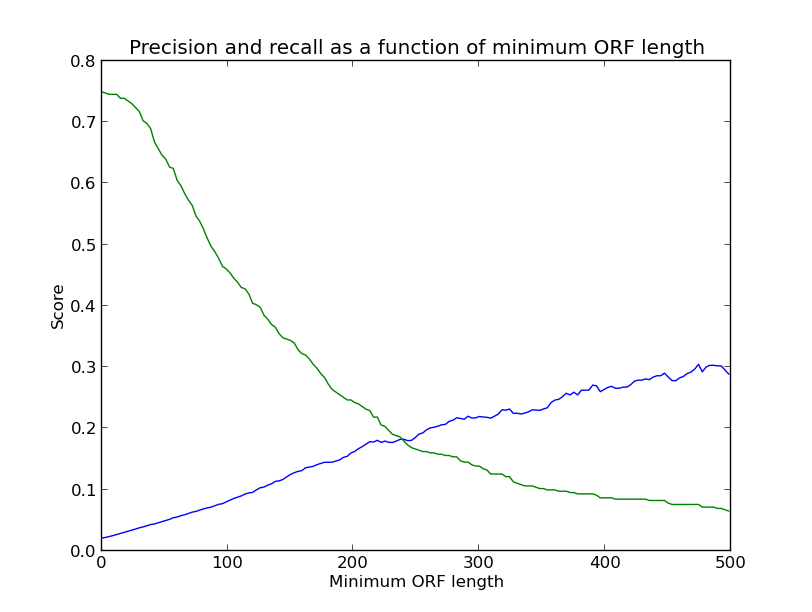
\includegraphics[scale=0.65]{precision-recall.png}
\caption{Blue line = precision. Green line = recall.}
\label{precrec}
\end{center}
\end{figure}

\subsection{Precision and recall for 125 codons or more}
0.1026 precision, 0.4017 recall

\subsection*{Emiliania huxleyi virus 86}

\subsubsection{Detecting ORFs}
2264 ORFs code for at least 60 amino acids.

\subsubsection{Precision and recall}
In Figure \ref{precrec2} we can see how precision and recall change depending on the minimum ORF length.
\begin{figure}[h!]
\begin{center}
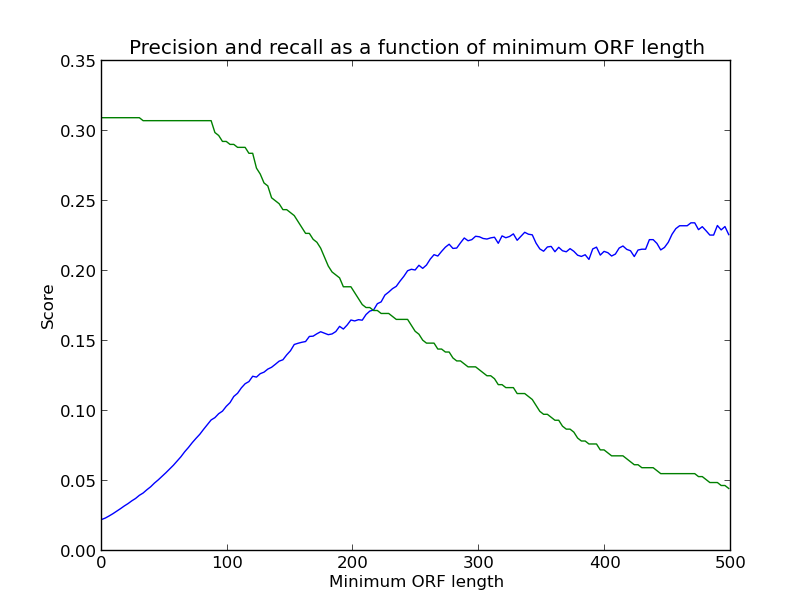
\includegraphics[scale=0.65]{precision-recall2.png}
\caption{Blue line = precision. Green line = recall.}
\label{precrec2}
\end{center}
\end{figure}
0.1254 precision, 0.2691 recall 

\section*{Honor Code}

% The following paragraph of your report should be included as is - do % not change it.

My answers to homework are my own work. I did not make solutions or code available to anyone else. I did not engage in any other activities that will dishonestly improve my results or dishonestly improve/hurt the results of others.

\end{document}